%%This is a very basic article template.
%%There is just one section and two subsections.
\documentclass{article}
\usepackage[utf8]{inputenc}
\usepackage[T1]{fontenc}
\usepackage[german]{babel}
\usepackage{blindtext}
\usepackage{graphicx}
\usepackage[colorlinks=true,linkcolor=black]{hyperref}
%\usepackage[obeyspaces]{url}
\newcommand*{\quelle}{% 
  \footnotesize Quelle: 
} 
\title{HappyWritter}
\date{2018\\Juli\\9}
\author{Lars Gächter\\ WISS}
\begin{document}
\maketitle
\clearpage
\tableofcontents
\clearpage 
\begin{abstract}
Dies ist eine kurze Zusammenfassung
\end{abstract}
\section{Einleitung}
\section{Anforderungen und Betriebsanleitung}
\subsection{Anforderungen}
Komplette WOnder Umgebung installiert\\
Java 8
\subsection{Getestete Funktionsfähigkeit}
Software\\
JRE JDK %1.8.0_171\\
\\
Java 8\\
MySQL MariaDB
\subsection{Betriebsanleitung}
Java Projekt
Kopiere oder entpacke den Ordner happywritter in den workspace Ordner von Eclipse.
Starte Eclipse und binde das Projekt happywritter ein.
Datenbank
Starte die Datenbank
Für das name.sql im 
\section{Datenbankmodellierung}
\subsection{ER-Modell}
\begin{figure}[h]
\begin{center}
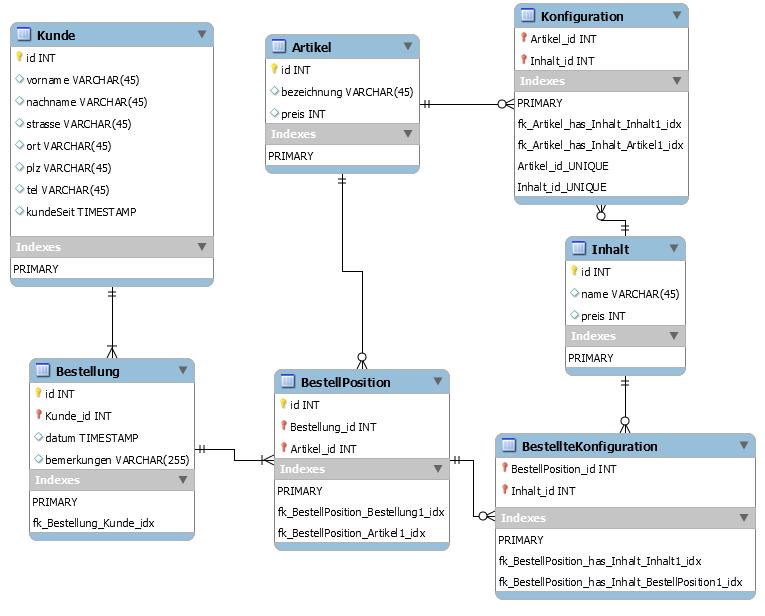
\includegraphics[width=0.7\textwidth]{res/erd.png}
\caption{ER-Modell}
\label{er-modell}
\end{center}
\end{figure}
\subsection{Entitäten und Attribute}
{\large Kunde}\\
Ist eine Person mit Vorname, Nachname, Strasse, Ort, Postleitzahl, Telefonnummer und Registrierdatum im System\\
\\
{\large Bestellung}\\
Datum der Bestellung, Bemerkung zur Bestellung\\
\\
{\large Bestell Position}\\
Trägt kein Attribut, ist für die Zuweisung eines Artikels für die Bestellung zuständig\\
\\
{\large Artikel}\\
Hat eine Bezeichnung und einen Preis\\
\\
{\large Inahlt}\\
Hat einen Namen und einen Preis 
\subsection{Beziehungen}
Speziell ist zu beachten, dass ein Artikel nicht in einer Bestell Position enthalten sein muss, um ein Artikel zu sein.\\
So ist auch eine Bestell Position immer noch eine Entität auch wenn diese in keiner Bestellkonfiguration vorkommt.\\
Damit aber Einträge in Bestell Position, Konfiguration und Bestellte Konfiguration valide sind, dürfen keine Referenzen nicht zugewiesen (null) sein.\\
\\
{\large Konfiguration}\\
Administrator vom Webshop kann bestimmen und strikt vorgeben, welche Beziehungen von Artikel und Inhalte eingegangen werden dürfen.\\
Damit bei der Konfiguration keine Duplikate entstehen würde sich ein Unique Index als nützlich erweisen.\\ 
\\
{\large Bestellte Konfiguration}\\
Der Kunde ist auch in der Lage Artikel mit Inhalte zu kombinieren, ist jedoch von den Konfigurationen des Administrators eingeschränkt.\\
Wenn der Kunde zu einem Artikel einen Inhalt mehrmals enthalten haben möchte, fehlt hier die die bestimmbare Anzahl von Inhalte, dies müsste redundante Einträge in der Bestellen Konfiguration erlauben.\\
\subsection{Abhängigkeiten}
Nicht abhängig sind Kunde, Artikel und Inhalt, welche unabhängig anderer Existenzen sind.
Für eine Konfiguration des Administrators benötigt es mindestens einen Artikel oder einen Inhalt, da diese null sein dürfen.\\
Für eine Bestellte Konfiguration des Kunden benötigt es mindestens eine Bestell Position oder einen Inhalt, da diese null sein dürfen.\\
Für eine Bestellung wird mindestens ein Kunde benötigt, welcher diese aufgegeben hat.\\
Eine Bestell Position benötigt und gehört genau zu einer Bestellung, kann aber ohne einen Artikel existieren, somit sind leere Bestellungen möglich.\\
Pro Bestell Position sind maximal ein Artikel möglich, so können auch existierende Artikel nicht in einer Bestell Position vorhanden sein, da kein Kunde diesen Artikel bisher bestellt hat.\\
\section{Klassendiagramm und Objekte}
\subsection{Klassendiagramm}
\begin{figure}[h]
\begin{center}
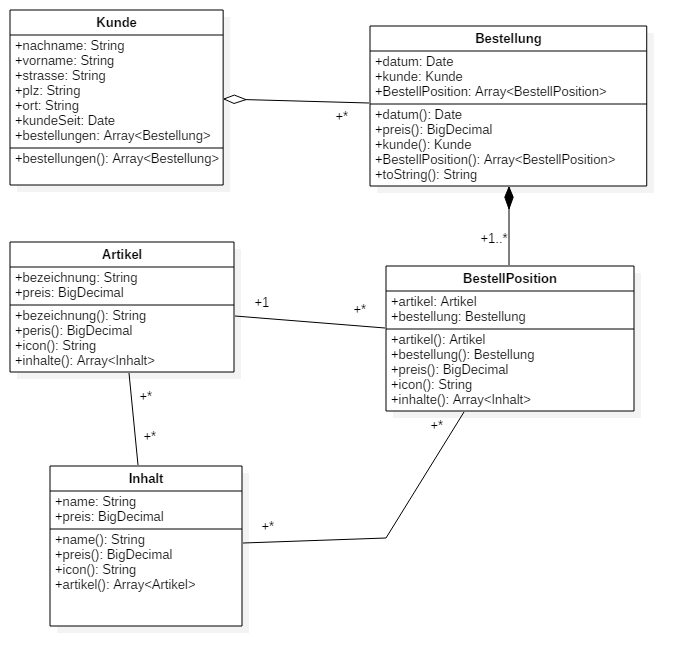
\includegraphics[width=0.7\textwidth]{res/uml.png}
\caption{Klassendiagramm}
\label{klassendiagramm}
\end{center}
\end{figure}
\subsection{Objekte}
Eigenschaften
Verhalten
\section{Projektordnerstruktur}
\subsection{Kurzbeschreibung}
Ordnername und Unterordnername
\subsection{Projektordner}
Hauptverzeichnis\\
\path{\happywritter}
\subsection{Resourcen Webapplikation}
Pfad
\path{\WebServerResources}
\subsection{Cascading Style Sheets}
Bootstrap\\
\path{\css}
\subsection{Bilder}
Artikel, Inhalte etc.\\
Pfad
\path{\img}
\subsection{Klassendiagramm Datei}
Pfad
\path{\uml}
\subsection{Datenbank Skript}
Der Skript für die Erstellung der Datenbank\\
Pfad
\path{\sql}
\subsection{ER-Modell}
Datenbankmodeldiagramm
Pfad
\path{\erd}
\subsection{Dokumentationen}
\path{\doc}\\
\path{\JavaDoc}\\
\path{\EOModel}\\
\path{\uml}\\
\path{\erd}
\subsection{Quellverzeichnis Java Klassen}
Session\\
Benutzer\\
Application\\
DirectAction\\
Pfad
\path{\Sources\ch\lars\your\app}\\
\\
Klassen Objekte aus dem eomodel generiert\\
Pfad
\path{\Sources\ch\lars\your\app\eomodel}\\
\\
Klassen für die Webkomponenten\\
Pfad
\path{\Sources\ch\lars\your\app\components}\\
\\
\subsection{EOModel}
Pfad
\path{\Resources}
\subsection{mysql Connector jar}
Pfad
\path{\Libraries}
\subsection{Komponenten}
Pfad
\path{\Components}
\subsection{Build der Klassen}
Pfad
\path{\bin}
\subsection{Build der WO Komponenten}
Pfad
\path{\build}
\section{Benutzungsanleitung}
\subsection{Administrator Login}
\subsection{Kunde Webshop}
\section{Quellenangabe}
mysql-workbench-plugin-doc-generating\\
\quelle\url{https://github.com/letrunghieu/mysql-workbench-plugin-doc-generating}\\
EOModelDoc\\
\quelle\url{https://wiki.wocommunity.org/display/WOL/EOModelDoc}
\end{document}\\